%%%%%%%%%%%%%%%%%%%%%%%%%%%%%%%%%%%%%%%%%%%%%%%%%%%%%%%%%%%%%%%%%%%%%%%%%%%%%
\section{Examples of OpencCL Applications}


%------------------------------------------------------------------------------
\subsection{OpenCL on FPGA platforms}

\subsubsection{OpenCL-FPGA Implementation}
As we already saw, OpenCL applications consists of two part: the host and the kernels.
FPGA flexibility allow the developer to opt for two solutions:

\begin{enumerate}
	\item An "`All in One"' solution, by implementing the CPU that will run the standard C/C++ host code directly as a soft CPU inside the FPGA.
	\item A separate solution, by using an external microprocessor for the host and by programming the FPGA to execute the kernels only.
	\end{enumerate}
	
Unlike CPUs and GPUs, where parallel threads can be executed on different cores, FPGAs offer a different strategy. Kernel functions can be transformed into dedicated and deeply pipelined \textbf{hardware circuits} that are inherently multithreaded using the concept of pipeline parallelism. Each of these pipelines can be replicated many times to provide even more parallelism than is possible with a single pipeline. This translates in an immediate boost in performance.\\
Figure \ref {fig:fpga_example} shows a simple example of how kernels are translated into separate \textbf{hardware pipelines}.
	
\begin{figurehere}
 \centering
 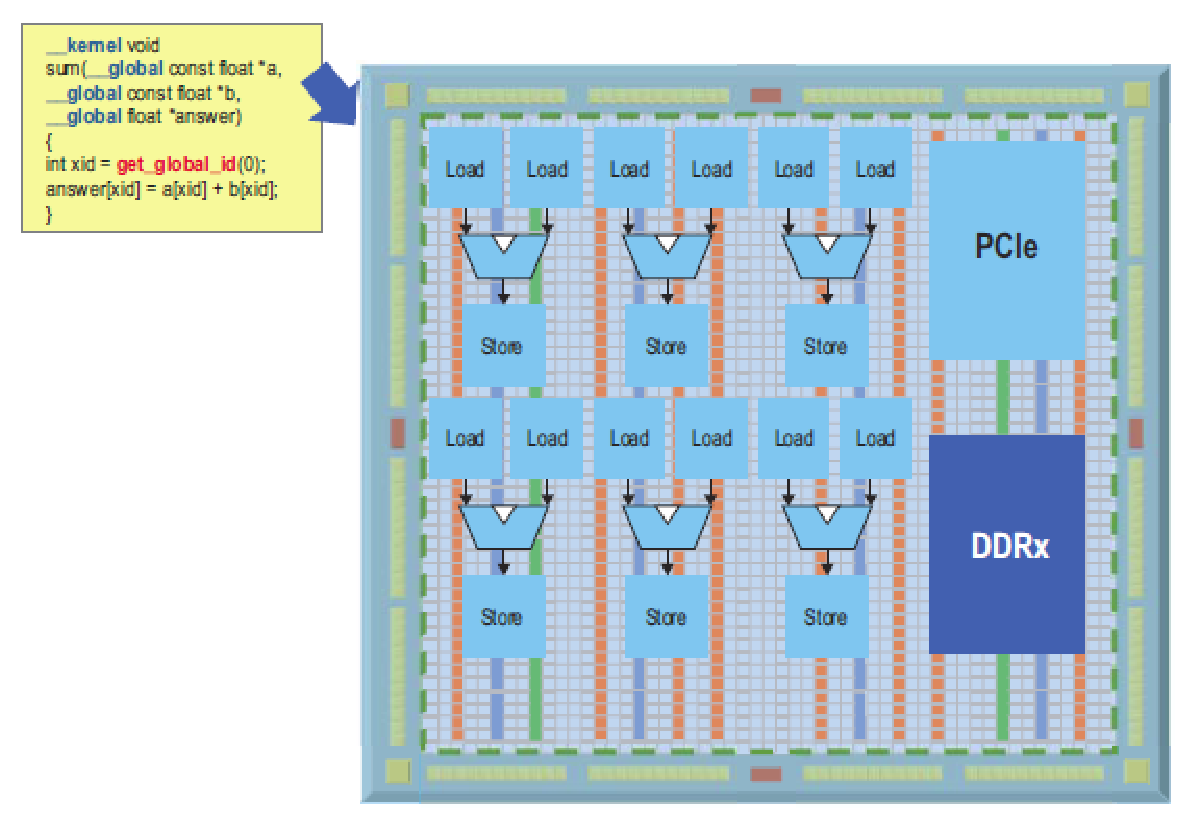
\includegraphics[width=8cm, height=4cm]{./eps/FPGA1.eps}
 \caption{FPGA implementation example}
 \label{fig:fpga_example}
\end{figurehere}

The most important concept behind the OpenCL-to-FPGA compiler is the notion of \textbf{pipeline parallelism}.
Basically, an OpenCL-to-FPGA compiler is able to implement the scenario observed in Section \ref{sect:pipelineScenario} in an automatic and more efficient way. We will describe how pipeline parallelism work by introducing an example, shown in Figure \ref{fig:fpga_example2}:

\begin{figurehere}
 \centering
 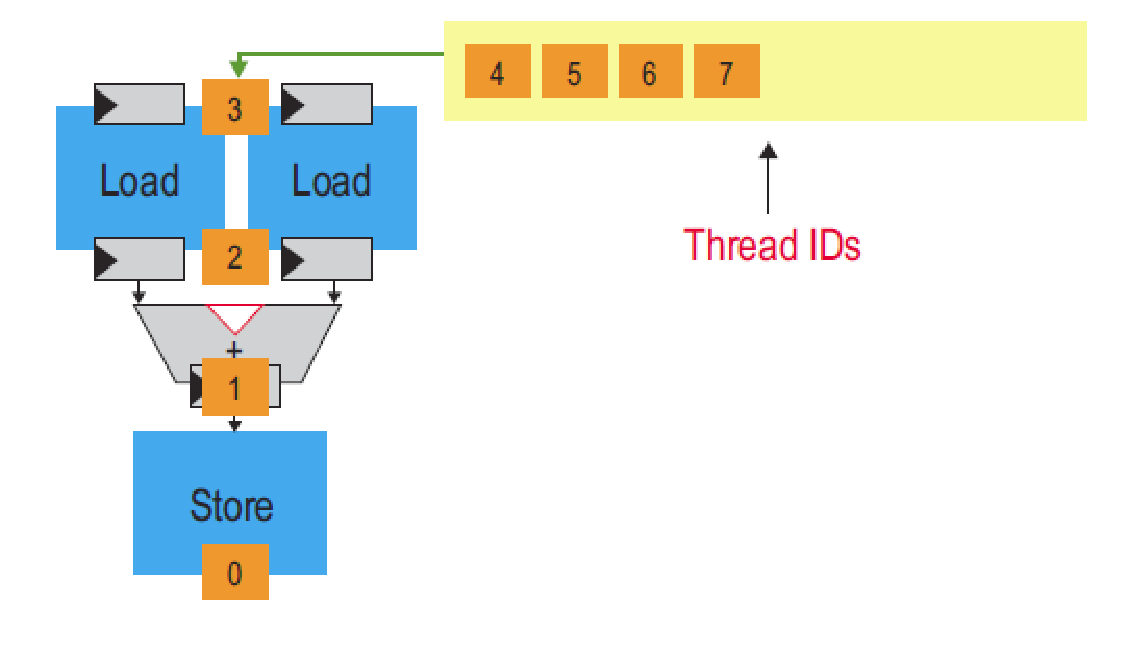
\includegraphics[width=8cm, height=4cm]{./eps/FPGA2.eps}
 \caption{Pipeline parallelism example}
 \label{fig:fpga_example2}
\end{figurehere}

On the first clock cycle, thread 0 is clocked into the two load units. This indicates that they should begin fetching the first elements of data from arrays A and B. On the second clock cycle, thread 1 is clocked in
at the same time that thread 0 has completed its read from memory and stored the results in the registers following the load units. On cycle 3, thread 2 is clocked in, thread 1 captures its returned data, and thread 0 stores the sum of the two values that it loaded. It is evident that in the steady state, all parts of the pipeline are active, with each stage processing a different thread.
	
To complete this section, we'll present a general scheme that summarize how OpenCL-FPGA applications are implemented (Figure \ref{fig:fpga_implementation}). One crucial point for parallel computation is the memory management, and as we can see from the figure several memory interfaces are needed, but luckily OpenCL-FPGA compilers are usually able to implement such interfaces automatically.

\begin{figurehere}
 \centering
 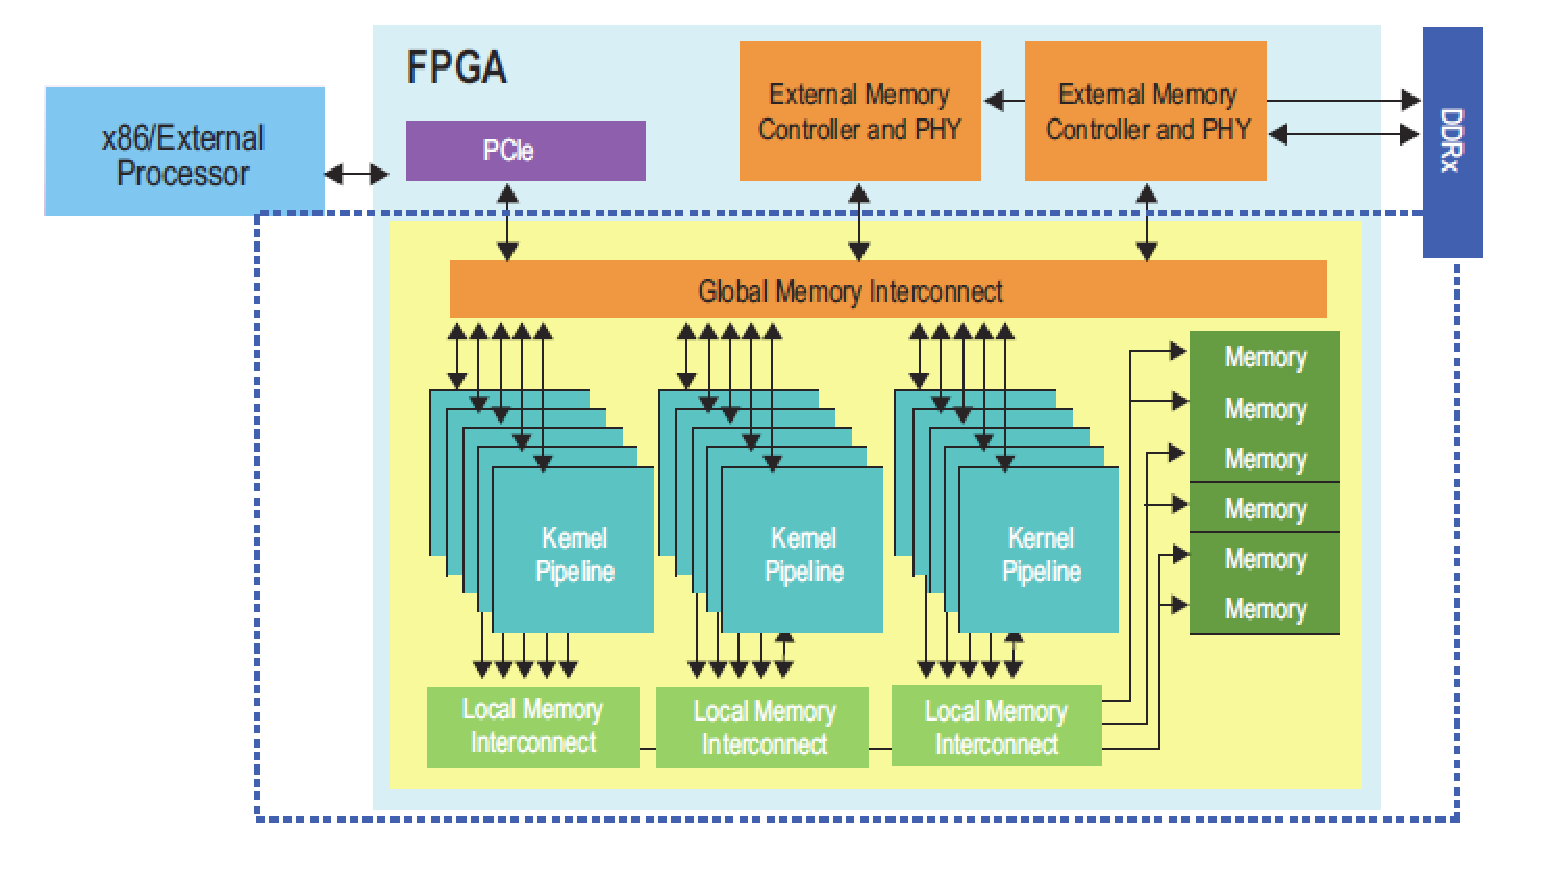
\includegraphics[width=8cm, height=4cm]{./eps/FPGA3.eps}
 \caption{OpenCL-FPGA Implementation scheme}
 \label{fig:fpga_implementation}
\end{figurehere}

\subsubsection{Benefits}

\begin{itemize}
	\item \textbf{Improved Time To Market:} OpenCL offers a quicker and simpler way to implement parallel alghorithms  compared to traditional FPGA development using lower level hardware description language (HDLs) such as Verilog or VHDL \cite {altera:FPGA}.  This because OpenCL inherently offers the ability to describe parallel computation, while the main challenge in HDLs languages was exactly to extract thread-level parallelism from a sequential program. OpenCL offers instead the ability to the programmer to explicitly specify and control parallelism.
	\item \textbf{Better Performance:} Dedicated ad-hoc hardware structures allow faster computation than using generic CPUs. Furthermore OpenCL-FPGA compilers exploit pipeline parallelism to make computation even faster.
	\item \textbf{Less Power Consumption:} Benchmarks show that FPGA applications consumes lot less power to execute the same OpenCL code in comparison to CPU or GPU.
\end{itemize}

\subsubsection{Case Study: Monte Carlo Black-Scholes Method}

In this experiment an economic model was used to benchmark an OpenCL-FPGA unit. The model is based on the 
Monte Carlo Black-Scholes method and it is used to compute the expected payoff of stock prices over millions of different paths. The entire algorithm used for this benchmark can be implemented in approximately 300 lines of
OpenCL code that is portable from FPGA to CPU to GPU, and we can see the comparison in performance on these 3 different platforms in Table \ref{tab:FPGABenchmark}.

\begin{tablehere}
{\footnotesize
\begin{tabular}{|p{1,0cm}|p{1,8cm}|p{1,8cm}|p{1,8cm}|}\hline
\textbf{Platform} & \textbf{Power} [Watts] & \textbf{Performance} [Billions of simulations per seconds] & \textbf{Efficiency} [Millions of sims per second per watt]\\ \hline
CPU & 130 & 0.032 & 0.0025 \\ \hline
GPU & 212 & 10.1 & 48 \\ \hline
FPGA & 45 & 12.0 & 266 \\ \hline
\end{tabular}}
  \caption{Monte Carlo Black-Scholes benchmark results\\}
	\label{tab:FPGABenchmark}
\end{tablehere}

As we can see, not only the OpenCL framework targeting a FPGA board exceeds the throughput of both a CPU and a GPU, but it also consumes one-fifth the power of comparable GPUs when executing the same code.

\subsubsection{Case Study: Document Filtering}

In this benchmark the focus is set on a more practical problem than the previous, as it will consider an algorithm used in modern data centers.
A recent report \cite{walsh:power} from International Data Corporation (IDC) examined the requirements of high performance computing data centers, and conducted a survey of the top constraints in expanding current data center capabilities. From the results, it was obvious that power and cooling costs are the key impediments of compute capability expansion, and as we have seen in the previous benchmark, FPGA computation offer an huge improvement in power consumption over CPUs and GPUs.\\
In this experiment, a document filtering algorithm was implemented using OpenCL, and it basically involves looking at an incoming stream of documents and finding the ones that best match a user's interest. The results are shown in Table \ref{tab:FPGABenchmark2}:

\begin{tablehere}
{\footnotesize
\begin{tabular}{|p{1,0cm}|p{1,8cm}|p{1,8cm}|p{1,8cm}|}\hline
\textbf{Platform} & \textbf{Power} [Watts] & \textbf{Performance} [Million of Terms per seconds] & \textbf{Efficiency} [Millions of Terms per Joule]\\ \hline
CPU & 130** & 2070 & 15.9 \\ \hline
GPU & 215 & 3240 & 15.1 \\ \hline
FPGA & 21 & 1755 & 83.6 \\ \hline
\end{tabular}}
  \caption{Document Filtering benchmark results\\ **Does not include memory consumption.}
	\label{tab:FPGABenchmark2}
\end{tablehere}

As we can see, although CPUs and GPUs can perform better in terms on throughput, the power efficiency of these two platform can be five time lower than the efficiency of FPGAs. It is interesting to note that in this case the performance of the FPGA was limited by the external memory bandwidth, and not by the FPGA itself. With a proper setup, the authors extimate a performance value of 2925 MT/s with the same power consumption, that would raise the power efficiency from 83.6 MT/J to 139,3 MT/J.
These results demonstrate that introducing an FPGA OpenCL implementation of algorithms, could bring a dramatic decrease of power consumption and thus cooling costs in modern data centers.


%-----------------------------------------------------------------------------

\subsection{TROVARE TITOLO}

In the next example \cite{Pennycook2012} we'll analyze how OpenCL was used to re-implement an existing benchmarking algorithm to (NO! IN REALTA' E' PIU' LENTO! Scopo: unico source??)damatically increase its performances. This example is interesting because it also analyzes how the introduction of Device Fission allow to obtain even more considerable speedups.

\subsubsection{Background: the LU algorithm}

LU is an application level benchmark part of the NPB Suite (NAS Parallel Benchmark) that consists in a series of parallel aerodynamic simulations designed by NASA. LU is short for Lower-Upper Gauss-Seidel solver and the algorithm is basically a simplified Navier-Stokes equation solver that uses three-dimensional data grid for its calculations. The size of these data cubes is always \begin{math}N^3\end{math}, and for the purpose of this example we'll focus only on three specific classes of problems: Class A problems (size \begin{math}64^3\end{math}), Class B problems (size \begin{math}102^3\end{math}) and Class C problems (size \begin{math}162^3\end{math}).
To perform the calculations, each cube of size (n X n X n) is divided into 2D "`slices"' of size (n X n X 1), and each "`slice"' is assigned to a different processor for computation. This algorithm is further optimized used a technique called \textit{k-blocking}; Figure \ref{dataCubes} shows a visual representation of how data is explored, as you can see each block must wait for the adjacent block to be completely computed (black blocks)before they can start.

\begin{figurehere}
 \centering
 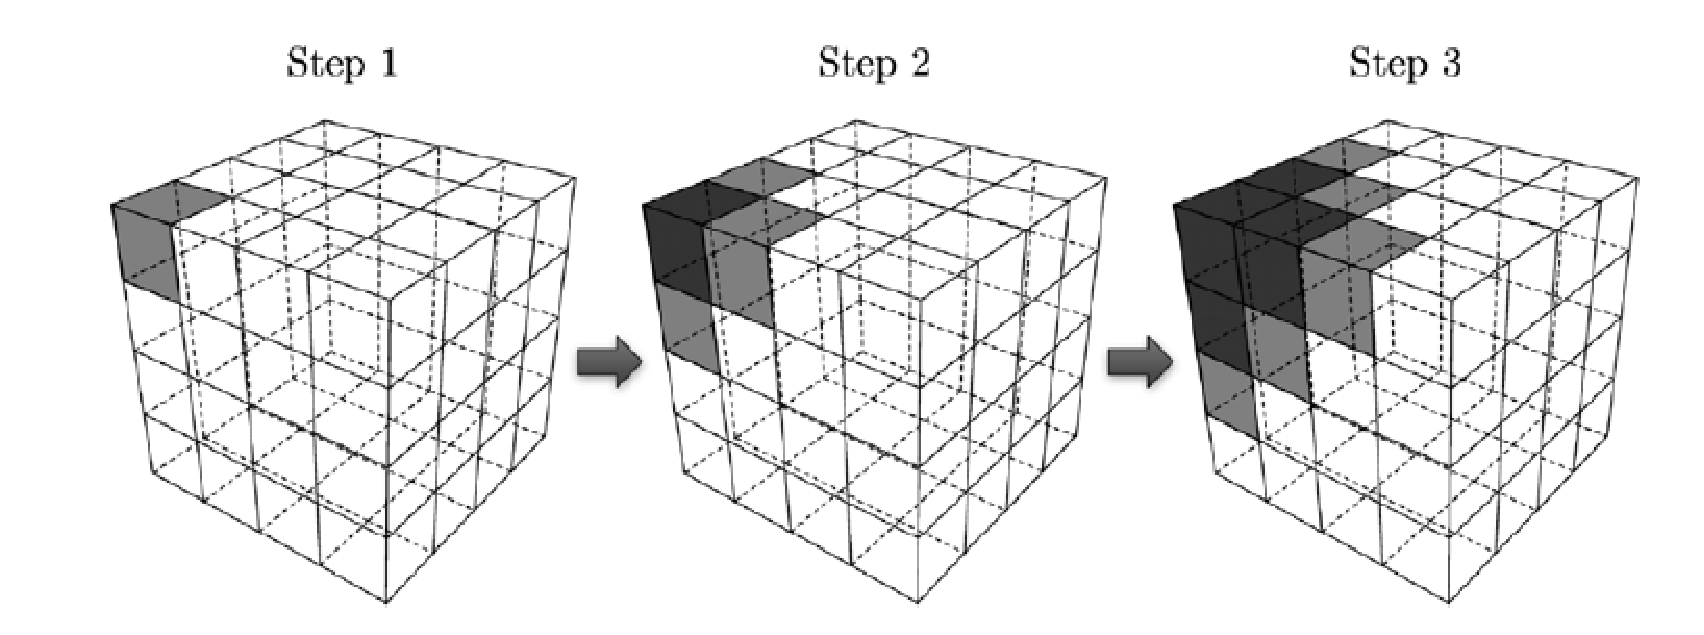
\includegraphics[width=8cm, height=4cm]{./eps/dataCube.eps}
 \caption{Data cubes used in the LU algorithm}
 \label{fig:dataCubes}
\end{figurehere}


\subsubsection{The Experiment}

\begin{tablehere}
{\footnotesize
\begin{tabular}{|p{2,2cm}|p{2,0cm}|p{2,0cm}|}\hline
\textbf{Platform} & \textbf{Compute Units} & \textbf{Processing Elements} \\ \hline
Intel X5550, 2.66 GHz (x86 CPU) & 4 & 4 \\ \hline
Intel X5660, 2.80 GHz (x86 CPU) & 12 & 12 \\ \hline
NVIDIA Tesla C1060 (GPU) & 30 & 240 \\ \hline
NVIDIA Tesla C2050 (GPU) & 14 & 448 \\ \hline
AMD/ATI FirePro V7800 (GPU) & 18 & 1440 \\ \hline
\end{tabular}}
  \caption{Platform used for the experiment}
	\label{tab:LUBenchmark1}
\end{tablehere}

Table \ref{tab:LUBenchmark1} shows a list of devices used in the experiment. One important aspect to note of OpenCl is its code portability: a single source can be used on different devices with different numbers of cores processing units, as OpenCL is able to scale automatically. This, for starters, already offers many benefits:

\begin{itemize}
	\item it is easier to maintain a single code that targets all platforms, as opposed to separate hand-tuned versions of the same code for each alternative platform.
	\item it reduces the risk of being locked into a single vendor solution.
	\item benchmarking is simplified, as the results can be compared from a single code source.
	\item it represents a "`safer"' investment for computing sites, as new codes (and ported legacy codes) will run on both existing and future architectures.
\end{itemize}

The goal of the experiment was to consider the performances of OpenCL implementation of LU against native FORTRAN77 (for CPUs) and CUDA (for GPUs). Figure \ref{fig:OpenCLvsFORTRAN77} shows the results for the comparison of the OpenCL implementation against the native FORTRAN77 implementation compiled using different compilers.

\begin{figurehere}
 \centering
 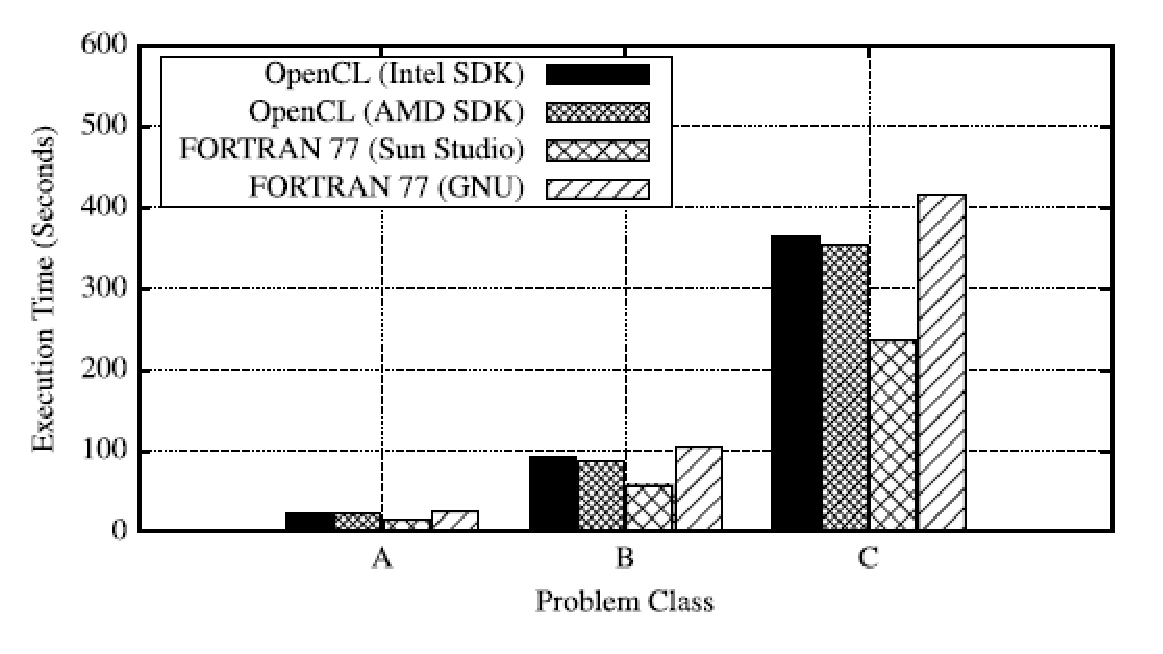
\includegraphics[width=8cm, height=4cm]{./eps/OpenCLvsFORTRAN77.eps}
 \caption{OpenCL vs Fortran Comparison}
 \label{fig:OpenCLvsFORTRAN77}
\end{figurehere}

As we can see the advantage of OpenCL (if any) is very marginal, and in the case of the Sun Studio compiler, the FORTRAN77 implementation performs way better. This result is very interesting because it demonstrates that \emph{OpenCL is not always the best option in term of performance}. The reason of this ``failure'' could be attributed to the fact that the FORTRAN compiler is very mature and has a long story of optimizations and fine-tuning behind it, while OpenCL standard is quite young.
Let's now see how OpenCL perform against another GPGPU implementation (CUDA), the results are shown in Figure \ref{fig:OpenCLvsCUDA}:

\begin{figurehere}
 \centering
 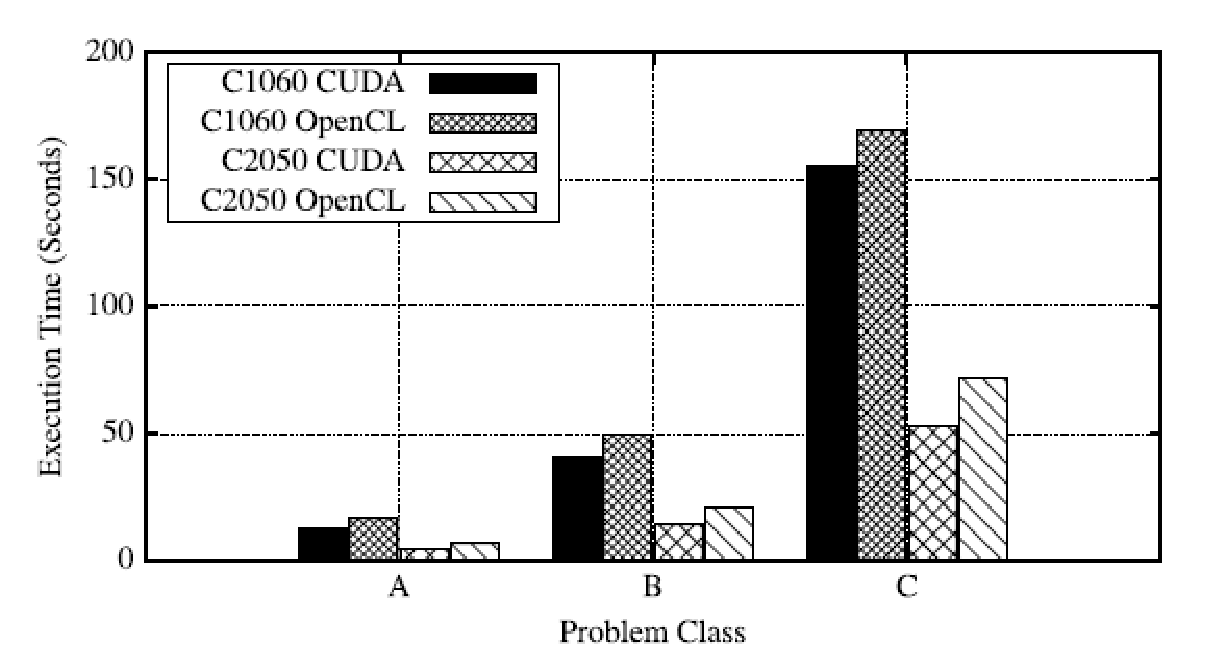
\includegraphics[width=8cm, height=4cm]{./eps/OpenCLvsCUDA.eps}
 \caption{OpenCL vs CUDA Comparison}
 \label{fig:OpenCLvsCUDA}
\end{figurehere}

As we can see even in this case the CUDA implementation performs a little better, and the reason in still to be searched into specific optimizations offered by the CUDA compiler for NVIDIA boards.

\subsubsection{Introducing Device Fission}

The same benchmark will now be ran using device fissioning to exploit either temporal or spatial cache locality and therefore use the shared memory in a more efficient way. Previous executions of the benchmark were unlikely to exhibit good memory behaviour, because basic OpenCL implementation has no control over which processing unit the work items will be allocated.
The LU benchmark will be executed over 2 different configurations created with device fissioning (Figure \ref{fig:LU_deviceFissionConfig}): two subdevices with 6 compute units each and 4 devices with 3 compute units each.

\begin{figurehere}
 \centering
 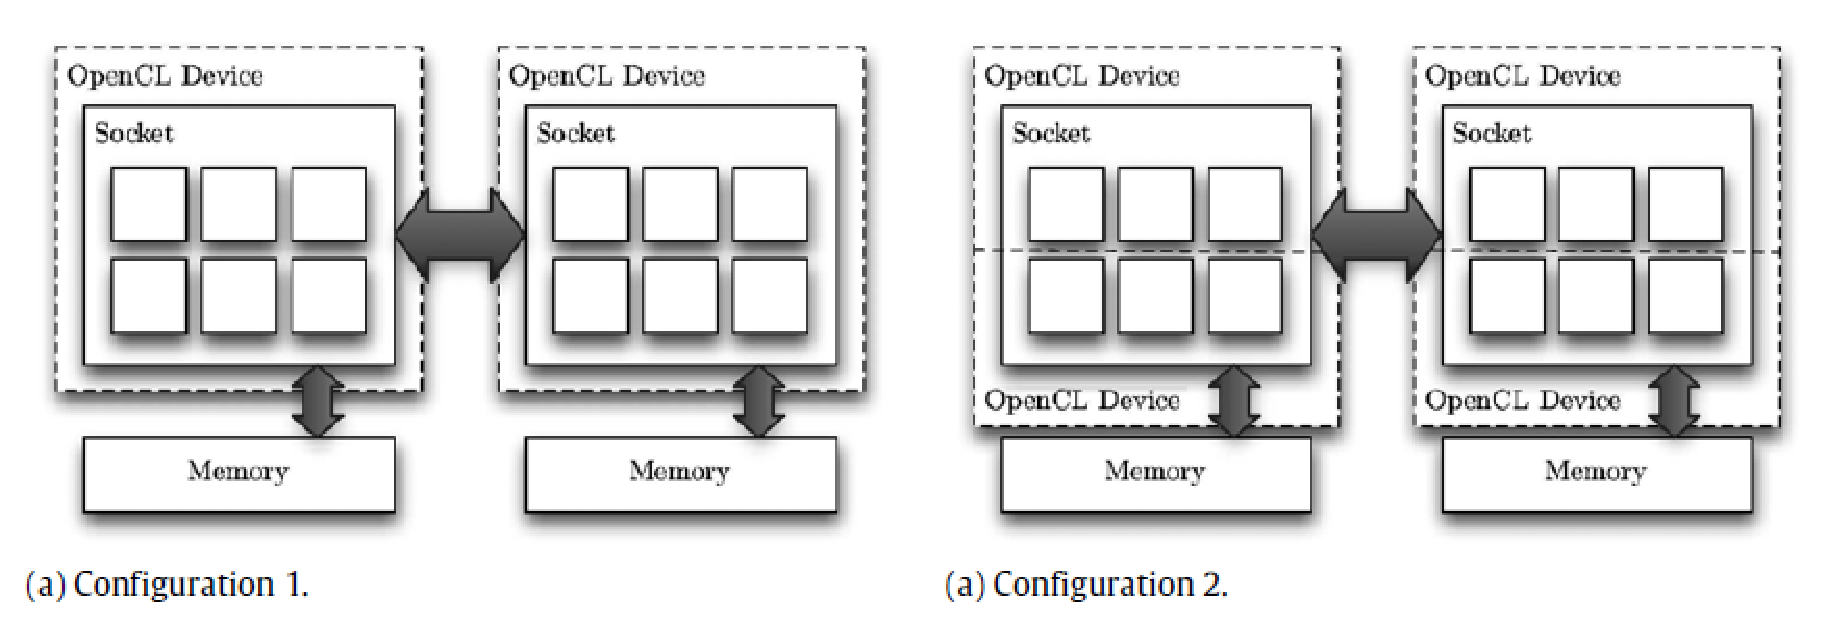
\includegraphics[width=8cm, height=4cm]{./eps/LU_deviceFissionConfig.eps}
 \caption{The configurations created with device fission}
 \label{fig:LU_deviceFissionConfig}
\end{figurehere}

The results of the test are listed in Table \ref{tab:LUDeviceFission}, and they clearly suggest that device fission can provide significant performance improvements when used and configured properly. \\

\begin{tablehere}
{\footnotesize
\begin{tabular}{|p{1,7cm}|p{1,7cm}|p{1,7cm}|p{1,7cm}|}
\hline
       Num of Cores		& \multicolumn{1}{|p{1,55cm}}{With Device Fission}& \multicolumn{1}{|p{1,55cm}}{Witout Device Fission}& \multicolumn{1}{|p{1,55cm}|}{Speedup} \\ \hline
\multicolumn{1}{|l}{Configuration 1} & \multicolumn{1}{c}{}  & \multicolumn{1}{c}{}  & \multicolumn{1}{c|}{}  \\ \hline
      24  & \multicolumn{1}{|c}{568.56} & \multicolumn{1}{|c}{1158.60} & \multicolumn{1}{|c|}{2.03x} \\ \hline
			48  & \multicolumn{1}{|c}{397.41} & \multicolumn{1}{|c}{760.73} & \multicolumn{1}{|c|}{1.92x} \\ \hline
      96  & \multicolumn{1}{|c}{276.68} & \multicolumn{1}{|c}{503.25} & \multicolumn{1}{|c|}{1.81x} \\ \hline
      384  & \multicolumn{1}{|c}{123.75} & \multicolumn{1}{|c}{n.a.} & \multicolumn{1}{|c|}{n.a.} \\ \hline

\multicolumn{1}{|l}{Configuration 2} & \multicolumn{1}{l}{}  & \multicolumn{1}{l}{}  & \multicolumn{1}{l|}{}  \\ \hline
      12  & \multicolumn{1}{|c}{622.27} & \multicolumn{1}{|c}{1884.87} & \multicolumn{1}{|c|}{3.02x} \\ \hline
			24  & \multicolumn{1}{|c}{394.63} & \multicolumn{1}{|c}{1158.60} & \multicolumn{1}{|c|}{2.93x} \\ \hline
      48  & \multicolumn{1}{|c}{250.84} & \multicolumn{1}{|c}{760.73} & \multicolumn{1}{|c|}{3.03x} \\ \hline
      192  & \multicolumn{1}{|c}{100.71} & \multicolumn{1}{|c}{320.53} & \multicolumn{1}{|c|}{3.18x} \\ \hline
\end{tabular}}
  \caption{Runtimes (in seconds) for two device fission configurations.}
	\label{tab:LUDeviceFission}
\end{tablehere}

%---------------------------------------------------------------------------------------------------

\subsection{OpenCL remote clustering}
In this section we'll present an interesting example \cite{mosix:virtualcl} about how OpenCL can be used in a distributed and \emph{heterogeneous} computer environment that can provide an opportunity to dramatically increase the performance of parallel and High-Performance Computing applications on clusters, by \emph{combining} traditional multi-core CPUs, general-purpose GPUs and Accelerator devices. One limitation of parallel computing using OpenCL is that most applications, run their device-specific code (the kernels) only locally on devices of the same computer were the hosts application runs.\\
Previous studies already demonstrated \cite{barak:heterogeneous} that OpenMP (one of the two main paradigms for HPC application developing) can be extended to use a heterogeneous cluster environment: while the CPU part of the application runs on one node, the GPU kernels run on cluster-wide devices.

\subsubsection{The VirtualCL Cluster Platform}
VirtualCL (VCL) is a wrapper developed by the authors of this study that allows most unmodified applications
to transparently utilize many OpenCL devices in a cluster as if all the devices are on the local computer.
The idea behind the platform is that it provides to the application the impression of a single host with many devices. Users can start a parallel application on a hosting computer, then VCL manages and transparently runs
the kernels of the application on different nodes.
VCL is composed of three main components: the VCL library, the broker and the back-end daemon.
The \textbf{VCL library} is a cluster-wide front-end for OpenCL that gives applications transparent access to cluster-wide openCL devices, hiding the actual location of the devices from the calling executable.
The \textbf{broker} is a daemon-process connected with the library via a UNIX socket that runs on every host computer. Its main tasks are to monitor for existence and availability of OpenCL devices in the cluster, to allocate them, and to authenticate and route messages between the applications and the back-ends.
While the brocker daemon runs on each host computer, the \textbf{back-end daemon} runs on each cluster node. Its goal is to run kernels on behalf of the client application.

\subsubsection{VCL Performances}
One of the main factors that have to be taken in account is the overhead introduced by the VCL model. To measure it it is sufficient to measure the time taken by an application to run a sequence of identical kernels using the native OpenCL library and the times to run the same kernels with VCL on local and remote devices; results are shown in Table \ref{tab:VCLOverhead} and it is clear that the difference between local and remote use of VCL is very small and almost independent from the size of the buffer used.\\

\begin{tablehere}
{\footnotesize
\begin{tabular}{|p{1,65cm}|p{1,65cm}|p{1,65cm}|p{1,65cm}|}\hline
\textbf{Buffer Size} & \textbf{Native OpenCL Time} [ms] & \textbf{VCL Overhead (Local)} [ms] & \textbf{VCL Overhead (Remote)} [ms]\\ \hline
4 KB & 96 & 35 & 113 \\ \hline
16 KB & 100 & 35 & 111 \\ \hline
64 KB & 105 & 35 & 106 \\ \hline
256 KB & 113 & 36 & 105 \\ \hline
1 MB & 111 & 34 & 114 \\ \hline
4 MB & 171 & 36 & 114 \\ \hline
16 MB & 400 & 36 & 113 \\ \hline
64 MB & 1354 & 33 & 112 \\ \hline
256 MB & 4993 & 37 & 111 \\ \hline
\end{tabular}}
  \caption{VCL overhead results.}
	\label{tab:VCLOverhead}
\end{tablehere}

The next step is to measure how VCL platform actually performs using benchmark applications. To run the test, applications from the SHOC (Scalable HeterOgeneous Computing) benchmark suite were used, and once again the execution time was measured first for native OpenCL implementation, and then for local and remote VCL implementation. The results are presented in Table \ref{tab:VCLBenchmark}.\\

\begin{tablehere}
{\footnotesize
\begin{tabular}{|p{1,65cm}|p{1,65cm}|p{1,65cm}|p{1,65cm}|}\hline
\textbf{Application} & \textbf{Native Time} [sec] & \textbf{VCL Time (Local)} [sec] & \textbf{VCL Time (Remote)} [sec]\\ \hline
BusSpeedDownload & 0.89 & 0.88 & 0.88 \\ \hline
BusSpeedReadback & 0.91 & 0.89 & 0.89 \\ \hline
DeviceMemory & 31.44 & 56.78 & 243.81 \\ \hline
KernelCompile & 5.91 & 5.93 & 5.94 \\ \hline
MaxFlops & 186.98 & 156.74 & 211.20 \\ \hline
QueueDelay & 0.88 & 0.93 & 1.22 \\ \hline
FFT & 7.29 & 7.15 & 7.33 \\ \hline
MD & 14.08 & 13.66 & 13.80 \\ \hline
Reduction & 1.60 & 1.58 & 2.88 \\ \hline
SGEMM & 2.11 & 2.13 & 2.43 \\ \hline
Scan & 2.53 & 2.54 & 6.57 \\ \hline
Sort & 0.98 & 1.04 & 1.53 \\ \hline
Spmv & 3.25 & 3.30 & 5.91 \\ \hline
Stencil2D & 11.65 & 12.48 & 18.94 \\ \hline
Triad & 6.01 & 11.83 & 53.37 \\ \hline
S3D & 32.39 & 32.68 & 33.17 \\ \hline
\end{tabular}}
  \caption{VCL benchmark results.}
	\label{tab:VCLBenchmark}
\end{tablehere}


By looking at the results it may seem that using VCL does not provide much advantage over native and local OpenCL implementation, but it is not to be forgotten that the goal was not to achieve better performances and faster execution, but rather to have remote and heterogeneous computation. Using cluster systems, much more computation power is available at the cost of network bandwidth and delay, so VCL has proven to perform better on applications with relatively long kernels and infrequent buffer-I/O operations, while those with many short kernels or with frequent or large I/O operations can't perform too well.
The opinion of the authors of this study is that running parallel kernels efficiently on remote devices in a cluster is quite feasible
and that VCL should be able to support largescale high-end parallel computing applications.
An ideal cluster for running parallel HPC applications with the VirtualCL platform would be a collection of low-cost servers, each with several OpenCL devices, connected by a low-latency, high-bandwidth network to high-end hosting nodes with many cores and large memories.








